%% Run LaTeX on this file several times to get Table of Contents,
%% cross-references, and citations.

\documentclass[11pt]{book}
\usepackage{gvv-book}
\usepackage{gvv}
%\usepackage{Wiley-AuthoringTemplate}
\usepackage[sectionbib,authoryear]{natbib}% for name-date citation comment the below line
%\usepackage[sectionbib,numbers]{natbib}% for numbered citation comment the above line

%%********************************************************************%%
%%       How many levels of section head would you like numbered?     %%
%% 0= no section numbers, 1= section, 2= subsection, 3= subsubsection %%
\setcounter{secnumdepth}{3}
%%********************************************************************%%
%%**********************************************************************%%
%%     How many levels of section head would you like to appear in the  %%
%%				Table of Contents?			%%
%% 0= chapter, 1= section, 2= subsection, 3= subsubsection titles.	%%
\setcounter{tocdepth}{2}
%%**********************************************************************%%

%\includeonly{ch01}
\makeindex

\begin{document}

\frontmatter
%%%%%%%%%%%%%%%%%%%%%%%%%%%%%%%%%%%%%%%%%%%%%%%%%%%%%%%%%%%%%%%%
%% Title Pages
%% Wiley will provide title and copyright page, but you can make
%% your own titlepages if you'd like anyway
%% Setting up title pages, type in the appropriate names here:

\booktitle{Signal Processing }

\subtitle{Through GATE}

\AuAff{G. V. V. Sharma}


%% \\ will start a new line.
%% You may add \affil{} for affiliation, ie,
%\authors{Robert M. Groves\\
%\affil{Universitat de les Illes Balears}
%Floyd J. Fowler, Jr.\\
%\affil{University of New Mexico}
%}

%% Print Half Title and Title Page:
%\halftitlepage
\titlepage

%%%%%%%%%%%%%%%%%%%%%%%%%%%%%%%%%%%%%%%%%%%%%%%%%%%%%%%%%%%%%%%%
%% Copyright Page

\begin{copyrightpage}{2024}
%Title, etc
\end{copyrightpage}

% Note, you must use \ to start indented lines, ie,
% 
% \begin{copyrightpage}{2004}
% Survey Methodology / Robert M. Groves . . . [et al.].
% \       p. cm.---(Wiley series in survey methodology)
% \    ``Wiley-Interscience."
% \    Includes bibliographical references and index.
% \    ISBN 0-471-48348-6 (pbk.)
% \    1. Surveys---Methodology.  2. Social 
% \  sciences---Research---Statistical methods.  I. Groves, Robert M.  II. %
% Series.\\

% HA31.2.S873 2004
% 001.4'33---dc22                                             2004044064
% \end{copyrightpage}

%%%%%%%%%%%%%%%%%%%%%%%%%%%%%%%%%%%%%%%%%%%%%%%%%%%%%%%%%%%%%%%%
%% Only Dedication (optional) 

%\dedication{To my parents}

\tableofcontents

%\listoffigures %optional
%\listoftables  %optional

%% or Contributor Page for edited books
%% before \tableofcontents

%%%%%%%%%%%%%%%%%%%%%%%%%%%%%%%%%%%%%%%%%%%%%%%%%%%%%%%%%%%%%%%%
%  Contributors Page for Edited Book
%%%%%%%%%%%%%%%%%%%%%%%%%%%%%%%%%%%%%%%%%%%%%%%%%%%%%%%%%%%%%%%%

% If your book has chapters written by different authors,
% you'll need a Contributors page.

% Use \begin{contributors}...\end{contributors} and
% then enter each author with the \name{} command, followed
% by the affiliation information.

% \begin{contributors}
% \name{Masayki Abe,} Fujitsu Laboratories Ltd., Fujitsu Limited, Atsugi, Japan
%
% \name{L. A. Akers,} Center for Solid State Electronics Research, Arizona State University, Tempe, Arizona
%
% \name{G. H. Bernstein,} Department of Electrical and Computer Engineering, University of Notre Dame, Notre Dame, South Bend, Indiana; formerly of
% Center for Solid State Electronics Research, Arizona
% State University, Tempe, Arizona 
% \end{contributors}

%%%%%%%%%%%%%%%%%%%%%%%%%%%%%%%%%%%%%%%%%%%%%%%%%%%%%%%%%%%%%%%%
% Optional Foreword:

%\begin{foreword}
%\lipsum[1-2]
%\end{foreword}

%%%%%%%%%%%%%%%%%%%%%%%%%%%%%%%%%%%%%%%%%%%%%%%%%%%%%%%%%%%%%%%%
% Optional Preface:

%\begin{preface}
%\lipsum[1-1]
%\prefaceauthor{}
%\where{place\\
% date}
%\end{preface}

% ie,
% \begin{preface}
% This is an example preface.
% \prefaceauthor{R. K. Watts}
% \where{Durham, North Carolina\\
% September, 2004}

%%%%%%%%%%%%%%%%%%%%%%%%%%%%%%%%%%%%%%%%%%%%%%%%%%%%%%%%%%%%%%%%
% Optional Acknowledgments:

%\acknowledgments
%\lipsum[1-2]
%\authorinitials{I. R. S.}  

%%%%%%%%%%%%%%%%%%%%%%%%%%%%%%%%
%% Glossary Type of Environment:

% \begin{glossary}
% \term{<term>}{<description>}
% \end{glossary}

%%%%%%%%%%%%%%%%%%%%%%%%%%%%%%%%
%\begin{acronyms}
%\acro{ASTA}{Arrivals See Time Averages}
%\acro{BHCA}{Busy Hour Call Attempts}
%\acro{BR}{Bandwidth Reservation}
%\acro{b.u.}{bandwidth unit(s)}
%\acro{CAC}{Call / Connection Admission Control}
%\acro{CBP}{Call Blocking Probability(-ies)}
%\acro{CCS}{Centum Call Seconds}
%\acro{CDTM}{Connection Dependent Threshold Model}
%\acro{CS}{Complete Sharing}
%\acro{DiffServ}{Differentiated Services}
%\acro{EMLM}{Erlang Multirate Loss Model}
%\acro{erl}{The Erlang unit of traffic-load}
%\acro{FIFO}{First in - First out}
%\acro{GB}{Global balance}
%\acro{GoS}{Grade of Service}
%\acro{ICT}{Information and Communication Technology}
%\acro{IntServ}{Integrated Services}
%\acro{IP}{Internet Protocol}
%\acro{ITU-T}{International Telecommunication Unit -- Standardization sector}
%\acro{LB}{Local balance}
%\acro{LHS}{Left hand side}
%\acro{LIFO}{Last in - First out}
%\acro{MMPP}{Markov Modulated Poisson Process}
%\acro{MPLS}{Multiple Protocol Labeling Switching}
%\acro{MRM}{Multi-Retry Model}
%\acro{MTM}{Multi-Threshold Model}
%\acro{PASTA}{Poisson Arrivals See Time Averages}
%\acro{PDF}{Probability Distribution Function}
%\acro{pdf}{probability density function}
%\acro{PFS}{Product Form Solution}
%\acro{QoS}{Quality of Service}
%\acro{r.v.}{random variable(s)}
%\acro{RED}{random early detection}
%\acro{RHS}{Right hand side}
%\acro{RLA}{Reduced Load Approximation}
%\acro{SIRO}{service in random order}
%\acro{SRM}{Single-Retry Model}
%\acro{STM}{Single-Threshold Model}
%\acro{TCP}{Transport Control Protocol}
%\acro{TH}{Threshold(s)}
%\acro{UDP}{User Datagram Protocol}
%\end{acronyms}

\setcounter{page}{1}

\begin{introduction}
This book provides solutions to signal processing problems in GATE.

\end{introduction}

\mainmatter

\chapter{Harmonics}
\chapter{Filters}
\chapter{ Z-transform}
\chapter{Systems}
\begin{enumerate}[label=\thechapter.\arabic*,ref=\thechapter.\theenumi]

\item Consider a unity-gain negative feedback system consisting of the plant $G\brak{s}$  and a proportional-integral controller. Let the proportional gain and integral
gain be 3 and 1, respectively. For a unit step reference input, the final values of the
controller output and the plant output, respectively, are
\begin{align}
    G\brak{s} = \frac{1}{\brak{s-1}} \notag
\end{align}\hfill (GATE EE 2023)\\
\solution 
% \iffalse
\let\negmedspace\undefined
\let\negthickspace\undefined
\documentclass[journal,12pt,twocolumn]{IEEEtran}
\usepackage{cite}
\usepackage{amsmath,amssymb,amsfonts,amsthm}
\usepackage{algorithmic}
\usepackage{graphicx}
\usepackage{textcomp}
\usepackage{xcolor}
\usepackage{txfonts}
\usepackage{listings}
\usepackage{enumitem}
\usepackage{mathtools}
\usepackage{gensymb}
\usepackage{comment}
\usepackage[breaklinks=true]{hyperref}
\usepackage{tkz-euclide} 
\usepackage{listings}
\usepackage{gvv}                                        
\def\inputGnumericTable{}                                 
\usepackage[latin1]{inputenc}                                
\usepackage{color}                                            
\usepackage{array}                                            
\usepackage{longtable}                                       
\usepackage{calc}                                             
\usepackage{multirow}                                         
\usepackage{hhline}                                           
\usepackage{ifthen}                                           
\usepackage{lscape}
\newtheorem{theorem}{Theorem}[section]
\newtheorem{problem}{Problem}
\newtheorem{proposition}{Proposition}[section]
\newtheorem{lemma}{Lemma}[section]
\newtheorem{corollary}[theorem]{Corollary}
\newtheorem{example}{Example}[section]
\newtheorem{definition}[problem]{Definition}
\newcommand{\BEQA}{\begin{eqnarray}}
\newcommand{\EEQA}{\end{eqnarray}}
\newcommand{\define}{\stackrel{\triangle}{=}}
\theoremstyle{remark}
\newtheorem{rem}{Remark}
\begin{document}
\parindent 0px

\bibliographystyle{IEEEtran}
\vspace{3cm}

\title{Assignment\\[1ex]GATE-EC-39}
\author{EE23BTECH11034 - Prabhat Kukunuri$^{}$% <-this % stops a space
}
\maketitle
\newpage
\bigskip

\renewcommand{\thefigure}{\theenumi}
\renewcommand{\thetable}{\theenumi}
\section{Question}
Consider the circuit shown in the figure with input V(t) in volts.The sinusoidal steady state current I(t) flowing through the circuit is shown graphically(where t is in seconds). The circuit element Z can be\rule{1.5cm}{0.15mm}.
\begin{enumerate}
    \item a capacitor of 1 F
    \item an inductor of 1 H
    \item a capacitor of $\sqrt{3}$ H
    \item an inductor of $\sqrt{3}$ H
\end{enumerate}
\begin{figure}[ht]
    \centering
    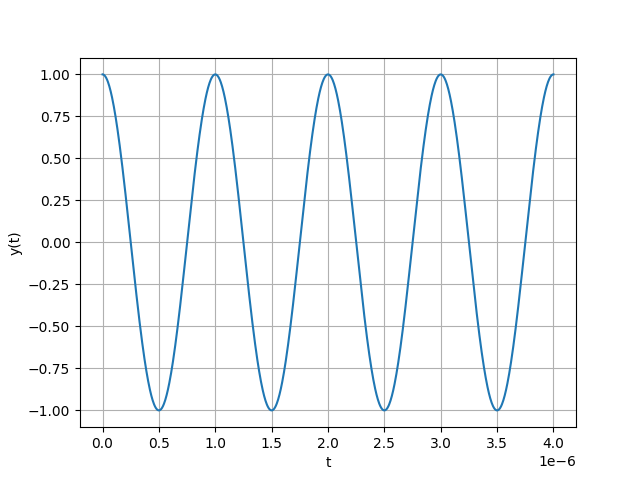
\includegraphics[width=\columnwidth]{figs/Figure_1.png}
    \label{fig:GATE.2022.EC.39.1}
\end{figure}
\solution\\
\begin{table}[h]
    \centering
    \begin{tabular}{|p{2cm}|p{2.80cm}|p{2.70cm}|}
    \hline
    Symbol&Value&Description\\ \hline
    $$x(n)$$&$$(x(0)+nd)u(n)$$&$$n^{th}$$ term of an A.P\\ \hline
    $$x(0)$$&$$x(0)$$&$1^{st}$ term of the A.P\\ \hline
    $$d$$&$$d$$&Common difference\\ \hline
    $$y(n)$$&$$x(n)\ast u(n)$$&Sum of n terms of an AP\\ \hline
    $$a$$&$$y(p-1)$$&Sum of first p terms of the AP\\ \hline
    $$b$$&$$y(q-1)$$&Sum of first q terms of the AP\\ \hline
    $$c$$&$$y(r-1)$$&Sum of first r terms of the AP\\ \hline
\end{tabular}
    \caption{Variable description}
    \label{tab:GATE.2022.EC.39.1}
\end{table}\\
The current through the circuit can be expressed as
\begin{align}
    I(t)=\sin\brak{t-\frac{\pi}{4}}
\end{align}
Since, the voltage seems to be leading the current the circuit element z is an inductor with inductance L.\\
Applying KVL in the circuit,
\begin{align}
    R.I\brak{t}+L\frac{dI\brak{t}}{dt}=sin\brak{t}
\end{align}
Applying Fourier transform to the differential equation,
\begin{align}
    &R.I\brak{s}+sL.I\brak{s}-\frac{1}{s^2+1}=0\\
    &I\brak{s}\brak{R+sL}=\frac{1}{s^2+1}\\
    &\sin\brak{at+b}\system{L}\frac{a\cos\brak{b}+s\sin\brak{b}}{a^{2}+s^{2}}\\
    &\sin\brak{t-\frac{\pi}{4}}\system{L}\frac{1-s}{2\brak{s^2+1}}\\
    &\frac{1-s}{2\brak{s^2+1}}\brak{R+sL}=\frac{1}{s^2+1}
\end{align}
Upon plugging in R=1$\ohm$,
\begin{align}
   L=\frac{1}{s}
\end{align}
Applying inverse Laplace,
\begin{align}
    L=1H
\end{align}

Appendix\\
Laplace transform of $\sin\brak{at+b}$ is as follows,
\begin{align}
    &\sin\brak{at+b}\system{L}\int_{0}^{\infty}\sin\brak{at+b}e^{-st}dt\\
    &\int_{0}^{\infty}\sin\brak{at+b}e^{-st}dt=\cos{b}\int_{0}^{\infty}\sin\brak{at}e^{-st}dt+\sin{b}\int_{0}^{\infty}\cos\brak{at}e^{-st}dt\\
    &\int_{0}^{\infty}\cos\brak{at}e^{-st}dt=\frac{e^{-st}}{a}sin{at}\Bigg|_{0}^{\infty}+\frac{s}{a}\int_{0}^{\infty}\sin\brak{at}e^{-st}dt\\
    &\int_{0}^{\infty}\cos\brak{at}e^{-st}dt=\frac{s}{a}\int_{0}^{\infty}\sin\brak{at}e^{-st}dt\label{eq:GATE.2022.EC.39.2}\\
    &\int_{0}^{\infty}\cos\brak{at}e^{-st}dt=\frac{s}{a}\brak{\frac{-e^{-st}}{a}cos{at}\Bigg|_{0}^{\infty}+\frac{s}{a}\int_{0}^{\infty}\cos\brak{at}e^{-st}dt}\\
    &\int_{0}^{\infty}\cos\brak{at}e^{-st}dt=\frac{s}{a^2}+\frac{s^2}{a^2}\int_{0}^{\infty}\cos\brak{at}e^{-st}dt
\end{align}
\begin{align}
    &\int_{0}^{\infty}\cos\brak{at}e^{-st}dt=\frac{s}{s^2+a^2},s>0
\end{align}
From \eqref{eq:GATE.2022.EC.39.2} we can say,
\begin{align}
    &\int_{0}^{\infty}\sin\brak{at}e^{-st}dt=\frac{a}{s^2+a^2},s>0\\
    &\therefore \sin\brak{at+b}\system{L}\frac{s\sin{b}+a\cos{b}}{s^2+a^2}
\end{align}
\end{document}

\newpage

\item Level \brak{h} in a steam boiler is controlled by manipulating the flow rate \brak{F} of the break-up(fresh) water using a proportional \brak{P} controller. The transfer function between the output and the manipulated input is   \\
$$ \frac{h\brak{s}}{F\brak{s}}=\frac{0.25\brak{1-s}}{s\brak{2s+1}} $$   \\
The measurement and the valve transfer functions are both equal to 1. A process engineer wants to tune the controller so that the closed loop response gives the decaying oscillations under the servo mode. Which one of the following is the CORRECT value of the controller gain to be used by the engineer? \\
\begin{enumerate}[label=(\alph*)]
    \item $0.25$
    \item $2$
    \item $4$
    \item $6$
\end{enumerate}

\solution
\newpage
\item \iffalse
\let\negmedspace\undefined
\let\negthickspace\undefined
\documentclass[journal,12pt,twocolumn]{IEEEtran}
\usepackage{cite}
\usepackage{amsmath,amssymb,amsfonts,amsthm}
\usepackage{algorithmic}
\usepackage{graphicx}
\usepackage{textcomp}
\usepackage{xcolor}
\usepackage{txfonts}
\usepackage{listings}
\usepackage{enumitem}
\usepackage{mathtools}
\usepackage{gensymb}
\usepackage{comment}
\usepackage[breaklinks=true]{hyperref}
\usepackage{tkz-euclide} 
\usepackage{listings}
\usepackage{gvv}                                        
\def\inputGnumericTable{}                                 
\usepackage[latin1]{inputenc}                                
\usepackage{color}                                            
\usepackage{array}                                            
\usepackage{longtable}                                       
\usepackage{calc}                                             
\usepackage{multirow}                                         
\usepackage{hhline}                                           
\usepackage{ifthen}                                           
\usepackage{lscape}
\usepackage{placeins}
\usepackage{xparse}


\newtheorem{theorem}{Theorem}[section]
\newtheorem{problem}{Problem}
\newtheorem{proposition}{Proposition}[section]
\newtheorem{lemma}{Lemma}[section]
\newtheorem{corollary}[theorem]{Corollary}
\newtheorem{example}{Example}[section]
\newtheorem{definition}[problem]{Definition}
\newcommand{\BEQA}{\begin{eqnarray}}
\newcommand{\EEQA}{\end{eqnarray}}
\newcommand{\define}{\stackrel{\triangle}{=}}
\theoremstyle{remark}
\newtheorem{rem}{Remark}

\graphicspath{ {./figs/} } 

\begin{document}

\bibliographystyle{IEEEtran}
\vspace{3cm}

\Large\title{GATE ME 30}
\large\author{EE23BTECH11032 - Kaustubh Parag Khachane $^{*}$% <-this % stops a space
}
\maketitle
\newpage
\bigskip

\renewcommand{\thefigure}{\theenumi}
\renewcommand{\thetable}{\theenumi}

\large\textbf{Question GATE ME 30} :\\
\fi
The figure shows a block of mass m = 20 kg attached to a pair of identical linear springs, each having a spring constant k = 1000 N/m. The block oscillates on a frictionless horizontal surface. Assuming free vibrations, the time taken by the block to complete ten oscillations is \rule{1cm}{0.15mm} seconds . (Rounded off to two decimal places) Take $\pi$ = 3.14.\hfill{GATE ME 30}

\begin{figure}[!ht]
\centering
\begin{center}
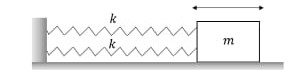
\includegraphics[width=\columnwidth]{2023/ME/30/figs/questiondiagram}
\end{center}
%\caption{Diagram for GATE ME Question 30}
\end{figure}


\item A system has transfer function
 \[\frac{Y(s)}{X(s)}=\frac {s-\pi}{s+\pi}\]
 let $u(t)$ be the unit step function.The input $x(t)$ that results in a steady-state output $y(t)=sin(\pi t)$ is \underline{\quad}.\hfill (GATE IN 2023)\\
 \solution
 \newpage
 
\end{enumerate}

\chapter{Sequences}
\begin{enumerate}[label=\thechapter.\arabic*,ref=\thechapter.\theenumi]

\item Consider the discrete time signal $x\sbrak{n} = u\sbrak{-n+5} - u\sbrak{n+3}$, where
\[u\sbrak{n} = 
\begin{cases}
    1;n\geq0\\
    0;n<0
\end{cases}
\]
The smallest n for which $x\sbrak{n} = 0$ is?
\\ \solution
\iffalse
\let\negmedspace\undefined
\let\negthickspace\undefined
\documentclass[journal,12pt,twocolumn]{IEEEtran}
\usepackage{cite}
\usepackage{amsmath,amssymb,amsfonts,amsthm}
\usepackage{algorithmic}
\usepackage{graphicx}
\usepackage{textcomp}
\usepackage{xcolor}
\usepackage{txfonts}
\usepackage{listings}
\usepackage{enumitem}
\usepackage{mathtools}
\usepackage{gensymb}
\usepackage{comment}
\usepackage[breaklinks=true]{hyperref}
\usepackage{tkz-euclide} 
\usepackage{listings}
\usepackage{gvv}                                        
\def\inputGnumericTable{}                                 
\usepackage[latin1]{inputenc}                                
\usepackage{color}                                            
\newtheorem{theorem}{Theorem}[section]
\usepackage{array}                                            
\usepackage{longtable}                                       
\usepackage{calc}                                             
\usepackage{multirow}                                         
\usepackage{hhline}                                           
\usepackage{ifthen}                                           
\usepackage{lscape}
\newtheorem{problem}{Problem}
\newtheorem{proposition}{Proposition}[section]
\newtheorem{lemma}{Lemma}[section]
\newtheorem{corollary}[theorem]{Corollary}
\newtheorem{example}{Example}[section]
\newtheorem{definition}[problem]{Definition}
\newcommand{\BEQA}{\begin{eqnarray}}
\newcommand{\EEQA}{\end{eqnarray}}
\newcommand{\define}{\stackrel{\triangle}{=}}
\theoremstyle{remark}
\newtheorem{rem}{Remark}
\begin{document}
\bibliographystyle{IEEEtran}
\vspace{3cm}
\title{GATE: IN/28}
\author{EE23BTECH11040 - Manoj Kumar Ambatipudi$^{*}$% <-this % stops a space
}
\maketitle
\newpage
\bigskip
\renewcommand{\thefigure}{\theenumi}
\renewcommand{\thetable}{\theenumi}
\textbf{QUESTION:}
Consider the discrete time signal $x\sbrak{n} = u\sbrak{-n+5} - u\sbrak{n+3}$, where
\[u\sbrak{n} = 
\begin{cases}
    1;n\geq0\\
    0;n<0
\end{cases}
\]
The smallest n for which $x\sbrak{n} = 0$ is?\\\hfill(GATE IN-2023)
\textbf{Solution:}
\fi
From \figref{IN/28/fig1}, the minimum value of $n$ is given as 
\begin{align}
    n = -3
\end{align}
\begin{figure}[h!]
\renewcommand\thefigure{1}
    \centering
    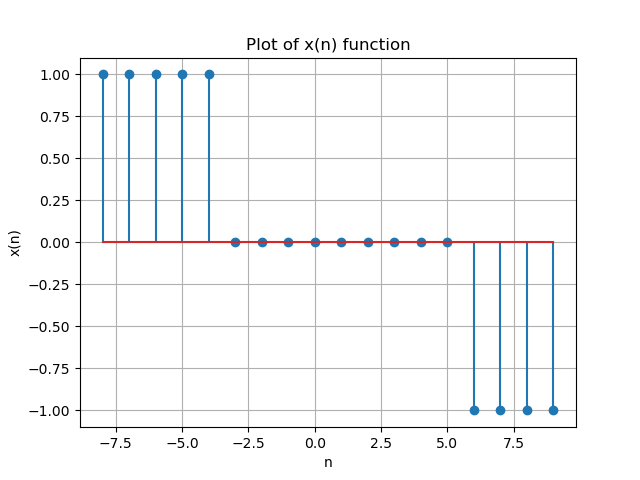
\includegraphics[width=1.0\columnwidth]{2023/IN/28/figs/fig_1.png}
    \caption{Plot of function $x\brak{n}$ taken from python3}
    \label{IN/28/fig1}
\end{figure}


\newpage

\end{enumerate}

\chapter{Sampling}
\begin{enumerate}[label=\thechapter.\arabic*,ref=\thechapter.\theenumi]

\item An $8$ bit ADC converts analog voltage in the range of $0$ to $+5\, V$ to the corresponding digital code as per the conversion characteristics shown in figure. For $V_{in} = 1.9922\, V$, which of the following digital output, given in hex, is true?

\begin{figure}[!h]
    \centering
    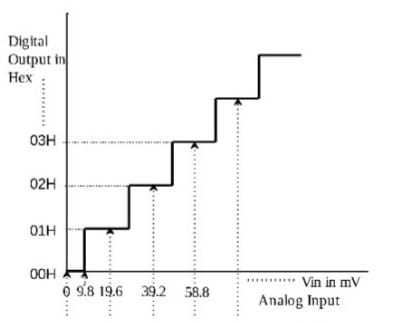
\includegraphics[width=\columnwidth]{2023/EE/40/figs/fig1.jpeg}
    \caption{}
    \label{fig:ADC_gate.ee.23.40}
\end{figure}
\begin{enumerate}[label=(\alph*)]
    \item $64H$
    \item $65H$
    \item $66H$
    \item $67H$
\end{enumerate} \hfill(GATE EE 40)

\solution
\iffalse
\let\negmedspace\undefined
\let\negthickspace\undefined
\documentclass[journal,12pt,twocolumn]{IEEEtran}
\usepackage{cite}
\usepackage{amsmath,amssymb,amsfonts,amsthm}
\usepackage{algorithmic}
\usepackage{graphicx}
\usepackage{textcomp}
\usepackage{xcolor}
\usepackage{txfonts}
\usepackage{listings}
\usepackage{enumitem}
\usepackage{mathtools}
\usepackage{gensymb}
\usepackage{comment}
\usepackage[breaklinks=true]{hyperref}
\usepackage{tkz-euclide} 
\usepackage{listings}
\usepackage{gvv}                                        
\def\inputGnumericTable{}                                
\usepackage[latin1]{inputenc}                            
\usepackage{color}                                       
\usepackage{array}                                       
\usepackage{longtable}                                   
\usepackage{calc}                              
\usepackage{tikz}
\usepackage{multirow}                                    
\usepackage{hhline}                                      
\usepackage{ifthen}                            
\usepackage{caption}
\usepackage{lscape}
\usepackage{amsmath}
\newtheorem{theorem}{Theorem}[section]
\newtheorem{problem}{Problem}
\newtheorem{proposition}{Proposition}[section]
\newtheorem{lemma}{Lemma}[section]
\newtheorem{corollary}[theorem]{Corollary}
\newtheorem{example}{Example}[section]
\newtheorem{definition}[problem]{Definition}
\newcommand{\BEQA}{\begin{eqnarray}}
\newcommand{\EEQA}{\end{eqnarray}}
\newcommand{\define}{\stackrel{\triangle}{=}}
\theoremstyle{remark}
\newtheorem{rem}{Remark}

\begin{document}

\bibliographystyle{IEEEtran}
\vspace{3cm}

\title{NCERT Math 11.9.2 Q8}
\author{EE23BTECH11009 - AROSHISH PRADHAN$^{*}$% <-this % stops a space
}
\maketitle
\newpage
\bigskip
\textbf{Question:} An $8$ bit ADC converts analog voltage in the range of $0$ to $+5\, V$ to the corresponding digital code as per the conversion characteristics shown in figure. For $V_{in} = 1.9922\, V$, which of the following digital output, given in hex, is true?

\begin{figure}[!h]
    \centering
    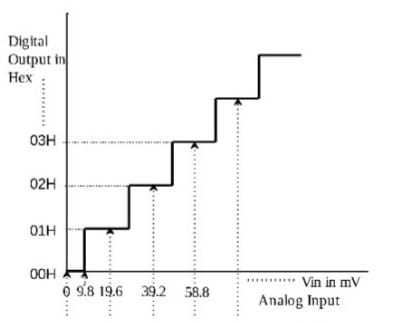
\includegraphics[width=\columnwidth]{2023/EE/40/figs/fig1.jpeg}
    \caption{}
    \label{fig:ADC_gate.23.ee.40}
\end{figure}
\begin{enumerate}[label=(\alph*)]
    \item $64H$
    \item $65H$
    \item $66H$
    \item $67H$
\end{enumerate}

\solution
\fi
\begin{table}[!h]
    \centering
    \resizebox{\columnwidth}{!}{\begin{tabular}{|p{2cm}|p{2.80cm}|p{2.70cm}|}
    \hline
    Symbol&Value&Description\\ \hline
    $$x(n)$$&$$(x(0)+nd)u(n)$$&$$n^{th}$$ term of an A.P\\ \hline
    $$x(0)$$&$$x(0)$$&$1^{st}$ term of the A.P\\ \hline
    $$d$$&$$d$$&Common difference\\ \hline
    $$y(n)$$&$$x(n)\ast u(n)$$&Sum of n terms of an AP\\ \hline
    $$a$$&$$y(p-1)$$&Sum of first p terms of the AP\\ \hline
    $$b$$&$$y(q-1)$$&Sum of first q terms of the AP\\ \hline
    $$c$$&$$y(r-1)$$&Sum of first r terms of the AP\\ \hline
\end{tabular}}
    \caption{Given Parameters}
    \label{tab:1_gate.23.ee.40}
\end{table}

Calculating the step-size:
\begin{align}
    \Delta V_{in} &= \frac{V_{max} - V_{min}}{2^n - 1}\\
    &= \frac{5 - 0}{2^8 - 1}\\
    &= \frac{5}{255}\\
   \implies V_{out} &= \frac{V_{in}}{\Delta V_{in}}\\
    &= \frac{1.9922 \times 255}{5}\\
    &= 101.59\\
    &\approx 102_{10}\\
    &= (66)_{H}
\end{align}
$\therefore$ correct answer is option (c).
\begin{figure}[!h]
    \centering
    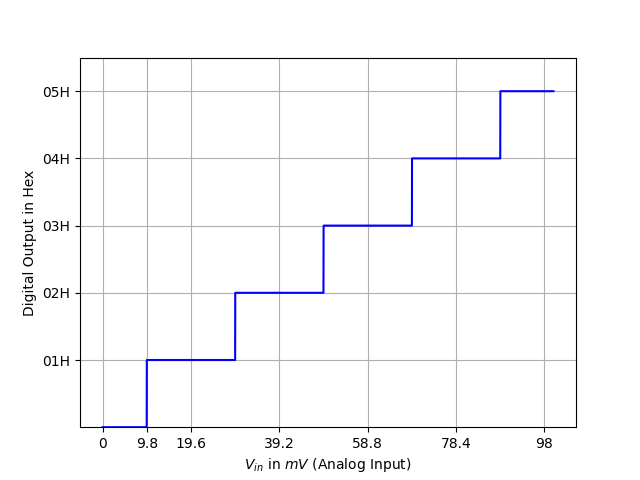
\includegraphics[width=\columnwidth]{2023/EE/40/figs/assign3.png}
    \caption{}
    \label{fig:ADC_plot_gate.23.ee.40}
\end{figure}
%\end{document}


\newpage

\end{enumerate}

\chapter{Contour Integration}
\chapter{Laplace Transform}
 \begin{enumerate}[label=\thechapter.\arabic*,ref=\thechapter.\theenumi]

\item The number of zeroes of the polynomial $P(s) = s^3+2s^2+5s+80$ in the right side of the plane?\hfill(GATE IN 2023) \\

\solution
% \iffalse
\let\negmedspace\undefined
\let\negthickspace\undefined
\documentclass[journal,12pt,twocolumn]{IEEEtran}
\usepackage{cite}
\usepackage{amsmath,amssymb,amsfonts,amsthm}
\usepackage{algorithmic}
\usepackage{graphicx}
\usepackage{textcomp}
\usepackage{xcolor}
\usepackage{txfonts}
\usepackage{listings}
\usepackage{enumitem}
\usepackage{mathtools}
\usepackage{gensymb}
\usepackage{comment}
\usepackage[breaklinks=true]{hyperref}
\usepackage{tkz-euclide} 
\usepackage{listings}
\usepackage{gvv}                                        
\def\inputGnumericTable{}                                 
\usepackage[latin1]{inputenc}                                
\usepackage{color}                                            
\usepackage{array}                                            
\usepackage{longtable}                                       
\usepackage{calc}                                             
\usepackage{multirow}                                         
\usepackage{hhline}                                           
\usepackage{ifthen}                                           
\usepackage{lscape}
\newtheorem{theorem}{Theorem}[section]
\newtheorem{problem}{Problem}
\newtheorem{proposition}{Proposition}[section]
\newtheorem{lemma}{Lemma}[section]
\newtheorem{corollary}[theorem]{Corollary}
\newtheorem{example}{Example}[section]
\newtheorem{definition}[problem]{Definition}
\newcommand{\BEQA}{\begin{eqnarray}}
\newcommand{\EEQA}{\end{eqnarray}}
\newcommand{\define}{\stackrel{\triangle}{=}}
\theoremstyle{remark}
\newtheorem{rem}{Remark}
\begin{document}
\parindent 0px

\bibliographystyle{IEEEtran}
\vspace{3cm}

\title{Assignment\\[1ex]GATE-EC-39}
\author{EE23BTECH11034 - Prabhat Kukunuri$^{}$% <-this % stops a space
}
\maketitle
\newpage
\bigskip

\renewcommand{\thefigure}{\theenumi}
\renewcommand{\thetable}{\theenumi}
\section{Question}
Consider the circuit shown in the figure with input V(t) in volts.The sinusoidal steady state current I(t) flowing through the circuit is shown graphically(where t is in seconds). The circuit element Z can be\rule{1.5cm}{0.15mm}.
\begin{enumerate}
    \item a capacitor of 1 F
    \item an inductor of 1 H
    \item a capacitor of $\sqrt{3}$ H
    \item an inductor of $\sqrt{3}$ H
\end{enumerate}
\begin{figure}[ht]
    \centering
    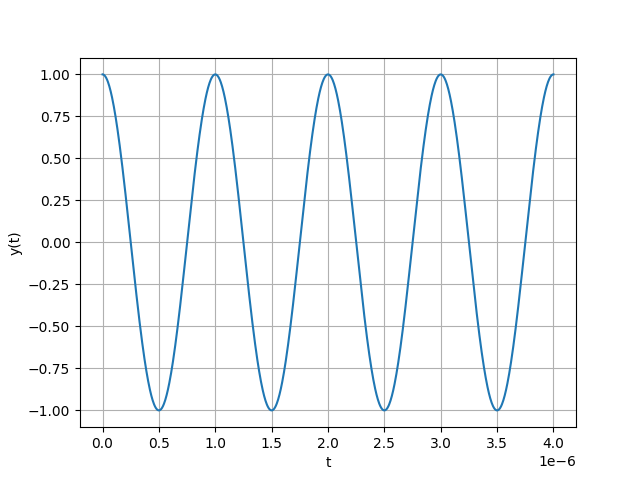
\includegraphics[width=\columnwidth]{figs/Figure_1.png}
    \label{fig:GATE.2022.EC.39.1}
\end{figure}
\solution\\
\begin{table}[h]
    \centering
    \begin{tabular}{|p{2cm}|p{2.80cm}|p{2.70cm}|}
    \hline
    Symbol&Value&Description\\ \hline
    $$x(n)$$&$$(x(0)+nd)u(n)$$&$$n^{th}$$ term of an A.P\\ \hline
    $$x(0)$$&$$x(0)$$&$1^{st}$ term of the A.P\\ \hline
    $$d$$&$$d$$&Common difference\\ \hline
    $$y(n)$$&$$x(n)\ast u(n)$$&Sum of n terms of an AP\\ \hline
    $$a$$&$$y(p-1)$$&Sum of first p terms of the AP\\ \hline
    $$b$$&$$y(q-1)$$&Sum of first q terms of the AP\\ \hline
    $$c$$&$$y(r-1)$$&Sum of first r terms of the AP\\ \hline
\end{tabular}
    \caption{Variable description}
    \label{tab:GATE.2022.EC.39.1}
\end{table}\\
The current through the circuit can be expressed as
\begin{align}
    I(t)=\sin\brak{t-\frac{\pi}{4}}
\end{align}
Since, the voltage seems to be leading the current the circuit element z is an inductor with inductance L.\\
Applying KVL in the circuit,
\begin{align}
    R.I\brak{t}+L\frac{dI\brak{t}}{dt}=sin\brak{t}
\end{align}
Applying Fourier transform to the differential equation,
\begin{align}
    &R.I\brak{s}+sL.I\brak{s}-\frac{1}{s^2+1}=0\\
    &I\brak{s}\brak{R+sL}=\frac{1}{s^2+1}\\
    &\sin\brak{at+b}\system{L}\frac{a\cos\brak{b}+s\sin\brak{b}}{a^{2}+s^{2}}\\
    &\sin\brak{t-\frac{\pi}{4}}\system{L}\frac{1-s}{2\brak{s^2+1}}\\
    &\frac{1-s}{2\brak{s^2+1}}\brak{R+sL}=\frac{1}{s^2+1}
\end{align}
Upon plugging in R=1$\ohm$,
\begin{align}
   L=\frac{1}{s}
\end{align}
Applying inverse Laplace,
\begin{align}
    L=1H
\end{align}

Appendix\\
Laplace transform of $\sin\brak{at+b}$ is as follows,
\begin{align}
    &\sin\brak{at+b}\system{L}\int_{0}^{\infty}\sin\brak{at+b}e^{-st}dt\\
    &\int_{0}^{\infty}\sin\brak{at+b}e^{-st}dt=\cos{b}\int_{0}^{\infty}\sin\brak{at}e^{-st}dt+\sin{b}\int_{0}^{\infty}\cos\brak{at}e^{-st}dt\\
    &\int_{0}^{\infty}\cos\brak{at}e^{-st}dt=\frac{e^{-st}}{a}sin{at}\Bigg|_{0}^{\infty}+\frac{s}{a}\int_{0}^{\infty}\sin\brak{at}e^{-st}dt\\
    &\int_{0}^{\infty}\cos\brak{at}e^{-st}dt=\frac{s}{a}\int_{0}^{\infty}\sin\brak{at}e^{-st}dt\label{eq:GATE.2022.EC.39.2}\\
    &\int_{0}^{\infty}\cos\brak{at}e^{-st}dt=\frac{s}{a}\brak{\frac{-e^{-st}}{a}cos{at}\Bigg|_{0}^{\infty}+\frac{s}{a}\int_{0}^{\infty}\cos\brak{at}e^{-st}dt}\\
    &\int_{0}^{\infty}\cos\brak{at}e^{-st}dt=\frac{s}{a^2}+\frac{s^2}{a^2}\int_{0}^{\infty}\cos\brak{at}e^{-st}dt
\end{align}
\begin{align}
    &\int_{0}^{\infty}\cos\brak{at}e^{-st}dt=\frac{s}{s^2+a^2},s>0
\end{align}
From \eqref{eq:GATE.2022.EC.39.2} we can say,
\begin{align}
    &\int_{0}^{\infty}\sin\brak{at}e^{-st}dt=\frac{a}{s^2+a^2},s>0\\
    &\therefore \sin\brak{at+b}\system{L}\frac{s\sin{b}+a\cos{b}}{s^2+a^2}
\end{align}
\end{document}

\newpage

\item The circuit shown in the figure is initially in the steady state with the switch K in open condition and $\overline{K}$ in closed condition. The switch K is closed and $\overline{K}$ is opened simultaneously at the instant $t = t_1$, where $t_1 > 0$. The minimum value of $t_1$ in milliseconds such that there is no transient in the voltage across the 100 $\mu F$ capacitor, is \rule{1cm}{0.15mm} (Round off to 2 decimal places) \hfill (GATE EE 2023)
    \begin{circuitikz}[american]
        \draw (0,7) to [R=10$\Omega$] (0,2) to [short] (3.5,2) to [isource, l={$\sin\brak{1000t}$}] (3.5,7) to [short] (0,7);
        \draw (3.5,2) to [short] (5,2) to [short] (5,0) to [R=$10\Omega$] (7.5,0) to [battery2 = 5V] (10,0) to [short] (10,2) to [curved capacitor=100$\mu$F, invert] (10,7) to [short] (5,7) to [short] (3.5,7);
        \draw (5,2) to [short] (7, 2) to[ospst=$\overline{K}$] ++(1,0);
        \draw (5,5) to [short] (5,2);
        \draw (10,2) to [short] (8,2);
        \draw (5,7) to [short] (5,6) to[cspst=K] ++(0,-1) ;
\end{circuitikz}


\newpage
\item $y=e^{mx}+e^{-mx}$ is the solution of which differential equation?
\begin{enumerate}[label=\textbf{\arabic*.}, font=\bfseries, align=left]
    \item $\frac{dy}{dx} - my = 0$ 
    \item $\frac{dy}{dx} + my = 0$ 
    \item $\frac{d^{2}y}{dx^{2}} + m^{2}y = 0$ 
    \item $\frac{d^{2}y}{dx^{2}} - m^{2}y = 0$ 
\end{enumerate} \hfill(GATE AG 2023)
\solution

\newpage
\item  A cascade control strategy is shown in the figure below. The transfer function between the output $(y)$ and the secondary disturbance $(d_2)$ is defined as  \\
$$G_{d2}(s)= \frac{y(s)}{d_2(s)}$$. 
Which one of the following is the CORRECT expression for the transfer function $G_{d2}(s)$? \\
\begin{figure}[h]
    \centering
    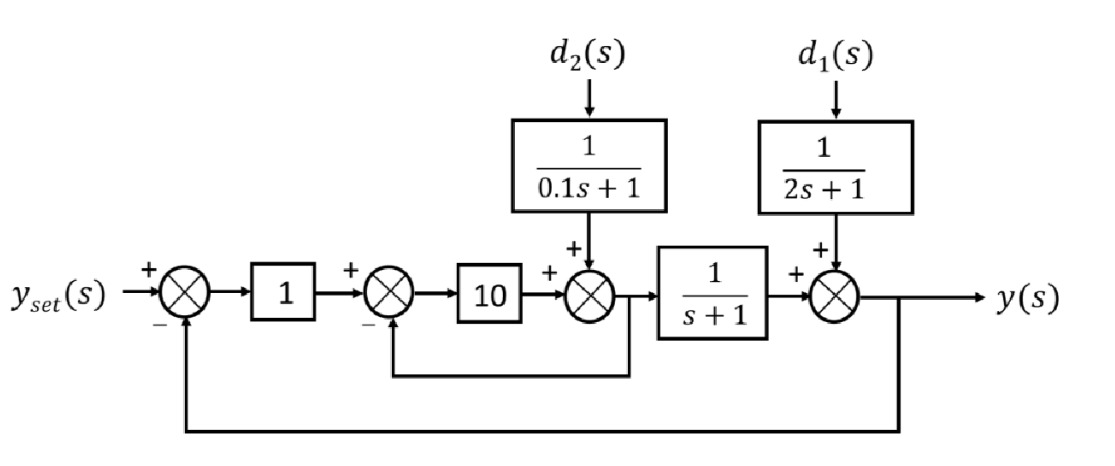
\includegraphics[scale=0.25]{2023/CH/44/figs/g44fig1.jpeg}
    \caption{ }
    \label{}
\end{figure}
\begin{enumerate}[label=\Alph*.]
\item $\frac{1}{(11s+21)(0.1s+1)}$ 
\item $\frac{1}{(s+1)(0.1s+1)}$
\item $\frac{(s+1)}{(s+2)(0.1s+1)}$
\item $\frac{(s+1)}{(s+1)(0.1s+1)}$
\end{enumerate} \hfill (GATE CH 2023)
\solution
\newpage
\item In the differential equation $\frac{dy}{dx} + \alpha x y = 0, \alpha$ is a positive constant. If $y = 1.0$ at
$x = 0.0$, and $y = 0.8$ at $x = 1.0$, the value of $\alpha$ is (rounded off to three decimal places).  \hfill(GATE CE 2023)
\solution
\end{enumerate}

\chapter{Fourier Transfrom}
 \begin{enumerate}[label=\thechapter.\arabic*,ref=\thechapter.\theenumi]
    \item The discrete-time Fourier transform of a signal x\sbrak{n} is $X\brak{\Omega}=\brak{1+\cos{\Omega}}e^{-j\Omega}$. Consider that $x_{p}\sbrak{n}$ is a periodic signal of period $N=5$ such that
        \begin{align}
            x_p\sbrak{n}&=x[n],\text{for n= 0, 1, 2}\\
            &=0,\text{for n= 3, 4}
        \end{align}
        Note that $x_p\sbrak{n}=\sum_{k=0}^{N-1}a_{k}e^{j\frac{2\pi}{N}kn}$. The magnitude of the Fourier series coefficient $a_3$ is \rule{3cm}{0.15mm} \brak{\text{Round off to 3 decimal places}}.\hfill(GATE EE 2023)
        \solution
        \newpage
\end{enumerate}
\backmatter
\appendix
\iffalse
\chapter{ Convolution}
\chapter{ Z-transform}
\fi
\latexprintindex

\end{document}

 
